
\section{Server}

En este apartado se busca hablar sobre el servidor, su arquitectura basada en microservicios usando docker, y docker-compose.

\subsection{Un viaje rapido por el servidor}

El servidor posee una arquitectura de microservicios Fig \ref{fig:server}, donde todos los servicios corren en Docker. Las barreras interactuan hacia el servicio de NestJS donde se suben los registros de entrada/salida, para luego procesar las imagenes (Solo en el caso del SL mini) mediante el servicio de Flask, para obtener la patente como texto. Los clientes pueden acceder a Grafana para visualizar datos tales como (DAR EJEMPLOS CUANDO ESTEN). La base de datos se mantiene aislada del exterior, por lo que no es posible acceder a ella directamente, y solo se puede interactuar mediante el servicio de NestJS.

\begin{figure}
        \centering
        
\includegraphics[width=.5\textwidth]{imgs/uncoma.png}
        \caption{Arquicetura del servidor}
        \label{fig:server}
\end{figure}

\subsection{Docker}

Docker es una plataforma de software que permite crear, probar e implementar aplicaciones mediante el uso de contenedores.

\subsubsection*{Contenedores}


Un contenedor de Docker funciona como una maquina virtual, practicamente aislada del sistema. La gran diferencia entre un contenedor y una maquina virtual es que el contenedor solo realiza una virtualización de capas por encima del sistema operativo, por lo que el contenedor comparte el kernel con el sistema padre, mientras que la maquina virtual emula todo incluido el kernel del sistema, esto produce que los contenedores sean más eficientes en el uso del hardware, pero altamente dependientes del kernel del sistema padre. Es por ello que un SO Windows no puede correr contenedores Linux de una forma sencilla y debe recurrir a una virtualización del kernel Linux Fig. \ref{fig:docker-funcinamiento}.


\begin{figure}
        \centering
        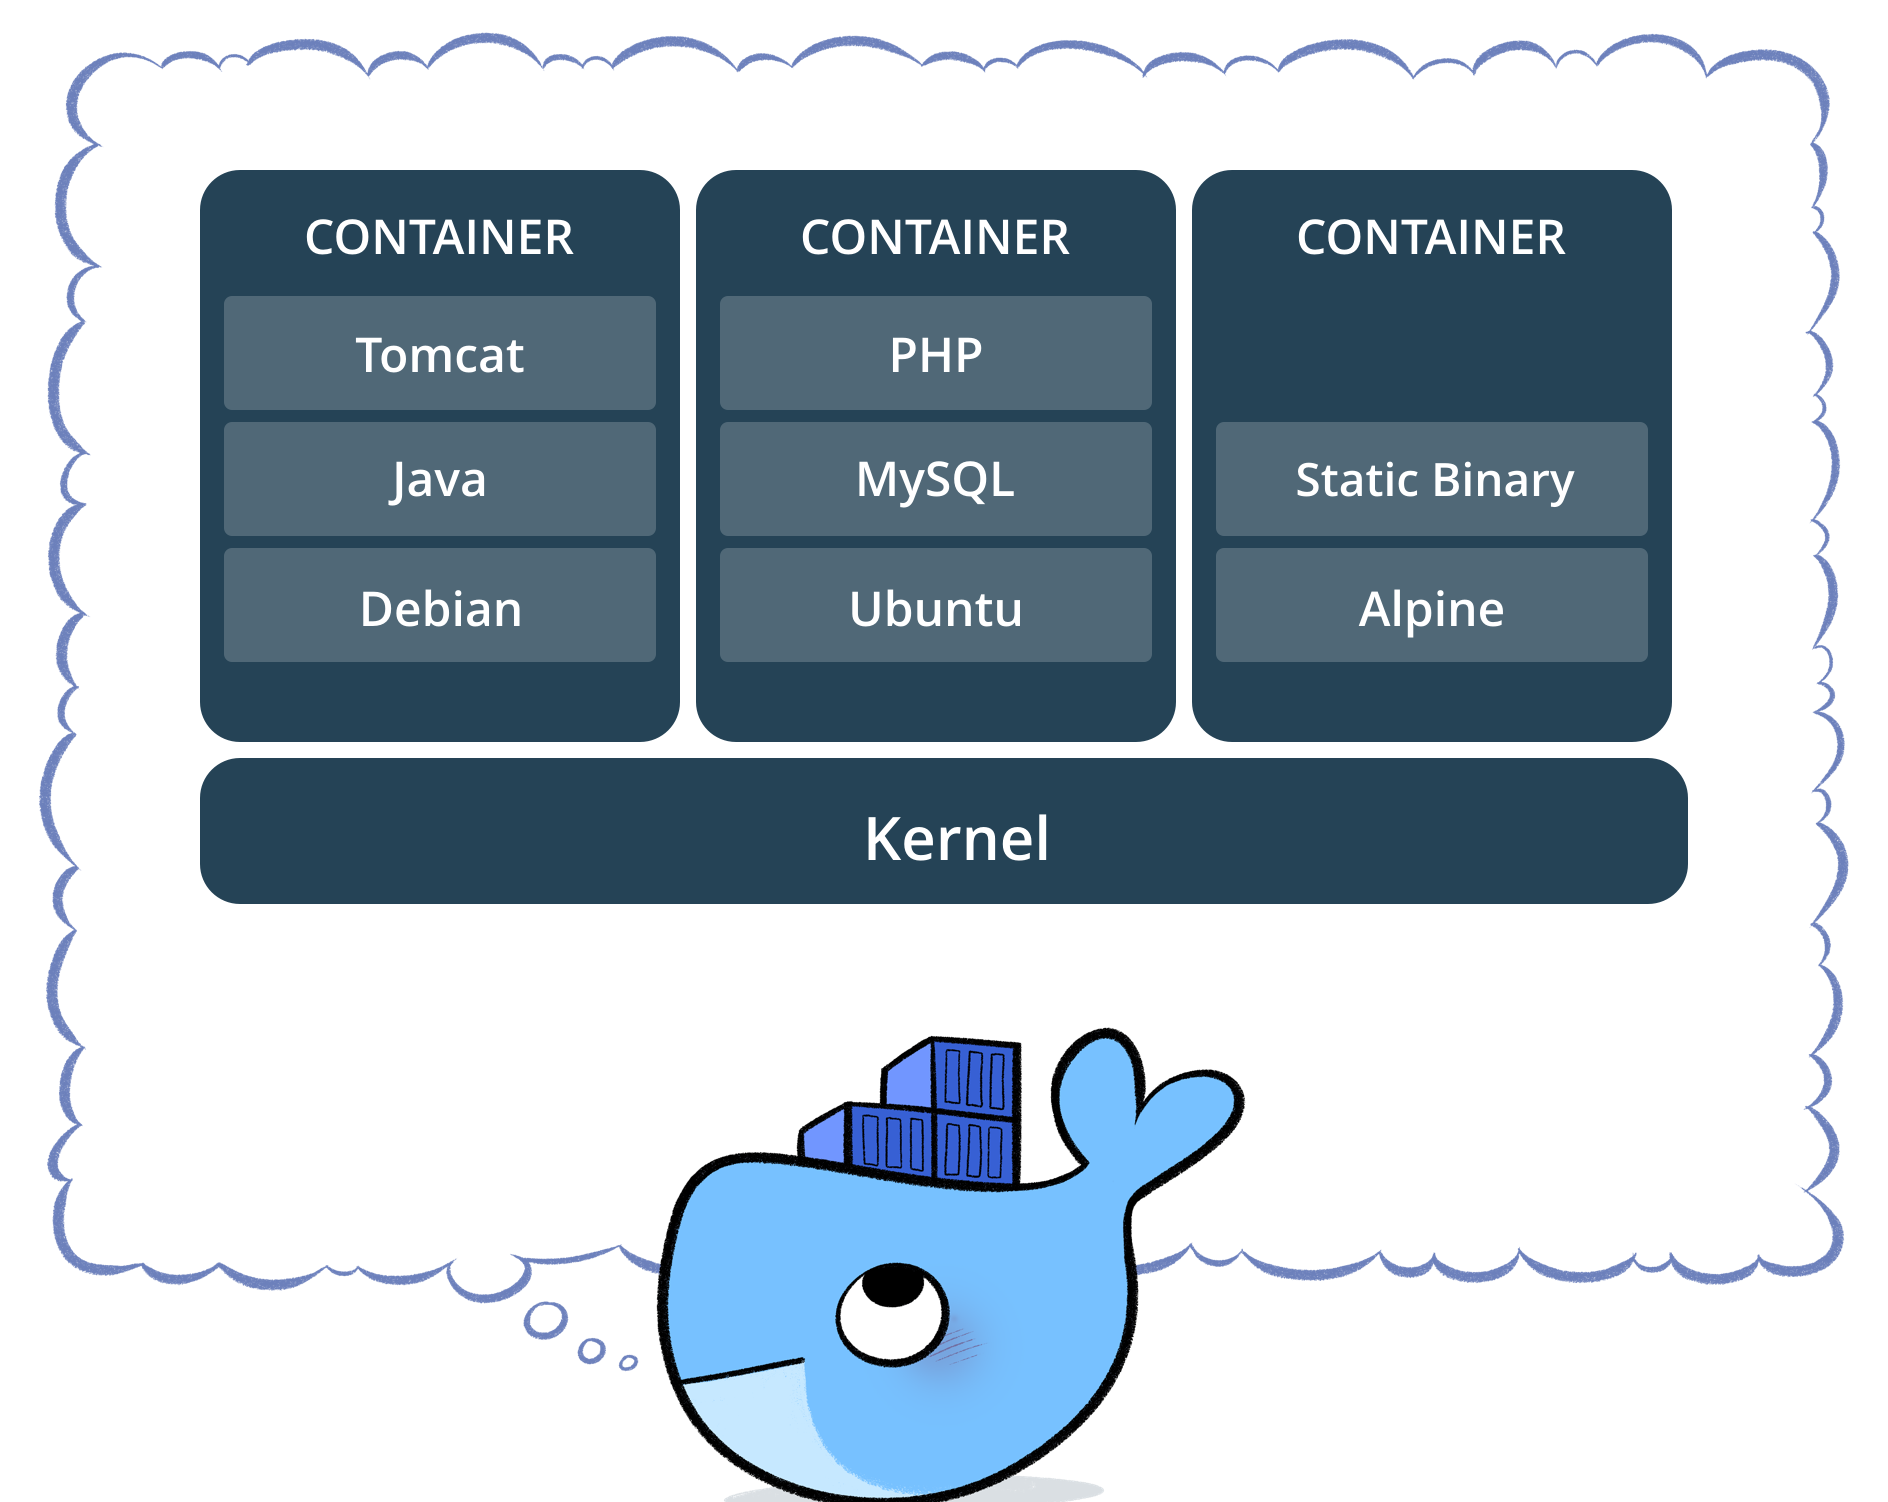
\includegraphics[width=.5\textwidth]{imgs/contenedores-docker.png}
        \caption{Funcionamiento de Docker}
        \label{fig:docker-funcinamiento}

\end{figure}

Una pregunta frecuente es: como guardo información que tengo en mi contenedor de docker en mi maquina? la solución a esta pregunta son los volumenes los cuales son un puente entre una carpeta de nuestra pc y una carpeta del contenedor, esto nos permite que cualquier archivo que contenga la carpeta de nuestra PC se encuentre en el contenedor, y viceversa. Esta comunicacíon entre el contenedor y nuestra PC nos permite realizar varias tareas, como realizar backups de la base de datos, compartir archivos de configuración para los diferente servicios.

\subsection{Docker compose}

A la hora de manejar varios contenedores el uso del interfaz de linea de comandos o CLI (por sus siglas en inglés) de Docker se vuelve engorrozo, es por ello que existen varios sistemas que tratan de simplificar y automatizar la tarea de levantar contenedores o servicios como los llamaremos de aquí en adelante. Una de estas tecnologías es Docker compose la cual permite definir dentro de un archivo yaml la arquitectura de los diferentes servicios [https://docs.docker.com/compose/], junto los volumenes y redes internas.

Cabe destacar que Docker compose crea una red interna en la cual (salvo que definamos de otra manera) todos los contenedores estan interconectados y podemos relacionarnos usando el nombre del servicio como url.

\subsection{Frontend vs Backend}

comparacion de los servicios frontend y backend explicando sus diferencias


\subsection{Microservicios}

La arquitectura de microservicios es una unión de servicios autónomos y pequeños. Esto nos permite que cada servicio utilice una tecnología diferente, siempre que sea necesario. En este trabajo se utiliza un servicio principal que utiliza NestJS (Javascript) y otro que utiliza Flask (Python), ya que Python posee una gran cantidad de herramienta para analisis de datos, mientras que Javascript junto con NestJS permite el desarrollo de un Backend mucho más confiable y rapido. Cada uno de estos servicios corre sobre un contenedor Docker indivual.

El servidor cuenta con los siguientes microservicios:

\begin{enumerate}
        \item Base de datos
        \item Applicacion backend con nestjs
              \subitem Usuarios
              \subitem Barreras
              \subitem Parques de estacionamiento
              \subitem Registros
        \item Frontend con ReactJS
        \item Applicacion backend con Flask (analisis de patente online)
\end{enumerate}


\subsection{Backend con NestJS}


Para la autenticación se utilizo el module de Passport JS, el cual permite crear estrategias para los diferentes tipos de autenticación, las estrategias utilizadas son:

\begin{enumerate}
        \item Local
        \item Apikey aplicaciones de terceros
        \item Apikey para las barreras
        \item JWT
\end{enumerate}

La estrategia Local, hace un logging del usuario segun su nombre de usuario y su contraseña.

Los servicios de apikey buscan que la apikey sea valida, es decir, se encuentre en la base de datos vinculada a una barrera, o este dentro de las apikeys validas de aplicaciones, en este caso solo 2 servicios se encuentran habilitados para realizar peticiones (Frontend y Grafana)

Un JSON Web Token es un estandar qué esta dentro del documento RFC 7519, este define un mecanismo para enviar información entre 2 partes, en este caso cliente-servidor de forma segura (utilizando cifrado). Los datos son codificados en un objeto de javascript (JSON),

\subsection{El cerebro de la aplicación}

Si bien, las barreras procesan datos antes de enviarlos, la logica del sistema se encuentra implementada en el server, corriendo bajo el servicio de NestJS, es decir el backend de nuestra app. Este servicio se encarga de interconectar la base de datos con lo requerido por los clientes, y las barreas. La idea es describir como maneja las peticiones mas importantes, que serian desde grafana, desde una app externa (como la pagina donde el usuario pide las barreras), y las peticiones de la misma barrera, siendo esta un apartado meramente tecnico de detalles de implementacion.


\subsection{Frontend con ReactJS}

Basicamente se va a hablar del panel admin y algun funciones para los clientes. junto con las librerias implementadas como ZOD,

\begin{enumerate}
        \item Manejo de estado global: https://docs.pmnd.rs/zustand/getting-started/comparison
        \item ZOD: https://zod.dev/
\end{enumerate}

Existen 2 clientes frontend uno para la adminitracion y otro para los clientes.

\subsubsection{Clientes}

La web para los clientes tienen una pagina de autenticación (ver figura), en esta web los clientes pueden darse de alta y entrar a su session, el manejo de la session se hace atravez de json web token, como fue nombrado en el apartado de backend.

En esta web los clientes pueden a los lugares que tiene a cargo, ya que se permite más de un lugar por usuario. Cada estacionamiento posee un panel para ver y configurar las barreras que posee, además cada barrera posee una descripción para que sea más sencillo que el usuario sepa a que barrera se refiere (hay que agregar figuras de como quedo la web). Los clientes pueden ver los registros de manera individual, asociados a cada lugar (figura de la web de registros y una figura del registro individual). La pagina más útil para sintetizar los datos es un panel de visualización de datos, el que permite ver horas totales utilizadas en el estacionamiento, y cantidad de autos, ambos graficos pueden ser trabajados por día, mes y año, ademas de poder filtrar por fechas (figura del dashboad).

\subsection{Mqtt broker}

Debido a la facilidad de manejar servicios en Docker, el broker mqtt que se utilizo es mosquito (documentación de mosquitto), como fue nombrado con anterioridad, este broker se encarga de conectar las barreras con el servidor backend. Actualmente el único topico que esta siendo utilizado es el de configuración de las barreras.

\subsection{Base de datos}

La base de datos del servicio es una base de datos no relacional basada en documentos [mongodb docs]. A la forma de los documentos en la base de datos se los denomina esquemas. Los esquemas que se implementaron fueron:

\begin{enumerate}
        \item Lugares
        \item Usuarios
        \item Barreras
        \item Datos de autenticación de las barreras
\end{enumerate}

La informacion que almacena cada documento, es decir, el esquema se muestra detalla acontinuación.




